% This is "bach-ref-2009.tex" Updated january 29th 2010.
% This file should be compiled with "sig-alternate-fixed.cls" January 2010.
% It is based on the ACM style "sig-alternate.cls"
% refers to the cls file being used
\documentclass{sig-alternate-br}
\usepackage{etoolbox}
\makeatletter
\patchcmd{\maketitle}{\@copyrightspace}{}{}{}
\makeatother
\usepackage{multirow}
\usepackage[utf8]{inputenc}
\usepackage{placeins} %place \FloatBarrier where the 
\usepackage{balance}
\usepackage{footnote}
\usepackage{tabularx}
\usepackage{xcolor}
\usepackage{array}
\usepackage{ctable}
\usepackage{lipsum} %dummy text
\newcolumntype{L}[1]{>{\raggedright\let\newline\\\arraybackslash\hspace{0pt}}m{#1}}
\pagenumbering{arabic}
\usepackage[hidelinks]{hyperref}

\begin{document}

\title{The Effect of Cooperation in Botnet-initiatives on the set-up of Control and Command Servers}
\numberofauthors{1}
\author{
\alignauthor
Sem Spenkelink\\
S1375490\\
       \affaddr{University of Twente}\\
       \affaddr{P.O. Box 217, 7500AE Enschede}\\
       \affaddr{The Netherlands}\\
       \email{j.s.spenkelink@student.utwente.nl}
}

\maketitle
\begin{abstract}
This paper describes an empirical research towards the effect of botnet-initiatives on the take-down of command and control servers. In particular, it focuses on the effectiveness of the take-down. We hypothesized that the effect prolongs after the take-down event has taken place. Secondly, we expected botnet-initiatives that feature a wider variety of organizations to perform better. Unfortunately, we did not find a significant difference in newly discovered C\&C's before and after the take-down. Therefore, it seems that botnet-initiatives do not alter the frequency botmasters set up new C\&C's.
\end{abstract}

\keywords{Zeus, Zbot, Botnet, Financial Malware, Cooperation, Information Sharing, Botnet-initiative}

\section{Introduction}
Botnets that distribute financial malware have shown to be an ever existing difficulty for crimefighters. The botnets themselves are maintained from various geographical locations, and the set-up of new control and command servers is becoming more accessible. To top that off the financial malware itself keeps changing and adapting against prevention or detection mechanisms. These critical infrastructure aspects of botnets make it difficult for law enforcement agencies to counteract the criminals. There are governmental issues, where it might be hard to be on one line with other governments regarding rules and regulations. These governments and law enforcement agencies often have little knowledge about the technological aspect of the botnets. Security companies that have the knowledge, often do not have the jurisdiction to act up. Furthermore, due to the nature of cyber-infrastructures, take-down of botnets may influence ongoing research or actions of third parties. To enhance the negative effects of botnet take-down it makes sense to cooperate, if possible globally, to take down criminals. Consequently, it is interesting to research the effect of botnet-initiatives where multiple parties work together against botnets or botmasters.

To elicit the problem and gain insight on what is already accomplished with collaborative botnet traceback, we start off with some literature review. The review is followed by establishing a research question with accessory hypotheses. We will work out this research question in the methodology and conclude with results and some discussion.

\section{Literature Review}
The detection of bots in a botnet network has been an ongoing field of research for quite some time. Previous research\cite{Keisuke2009400,Zhaosheng2008967} has shown that there are effective strategies against the detection and traceback of botnets. Nonetheless, these botnets remain a vast problem as these techniques are not deployed by leading organizations such as ISPs. Houmansadr and Borisov\cite{Houmansadr2013707} have developed a way for end-users or organizations to work around this discrepancy. They use a watermark to detect infected bot hosts. Even though this low-cost method of detection is of value to the organizations (mostly aimed at service providers), it still leaves the botnets running and it provides no global protection unless the traceback is enforced by governments. The method also has some discrepancies regarding more complex botnets. For example botnets using peer-to-peer structures or botnets that evade watermarks by adapting the flow structures of the network.
Evidently, all these methods lack collaboration between the hosts that have been hijacked and become C\&C's. In \cite{Mizoguchi2011639} researchers describe that including collaboration from these hosts can be a vital point in tracing down the C\&C's and eventually the botmaster. As we have established before, botnets of financial malware like Zeus can rely on more complex peer-to-peer networks (Figure \ref{fig:zeusarchitecture}). However, ongoing research has even enabled us to overcome the difficulty of these complex structures by means of information sharing\cite{Wang2014132}. The above research has clarified that information sharing is key to botnet traceback. It would make sense to see the effect of these efforts back in real life situations. Therefore, it is interesting to see how botnet-initiatives perform and if they actually provide us real life benefits for future reference. 

\begin{figure}[!h]
	\centering
    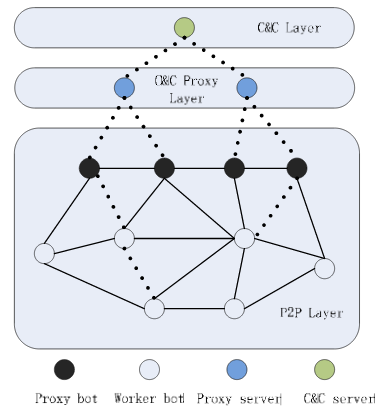
\includegraphics[width=\columnwidth,height=7.5cm,keepaspectratio]{zeusp2p.png}
    \caption{Zeus P2P Architecture\cite{Wang198273490}}
    \label{fig:zeusarchitecture}
\end{figure}

\FloatBarrier

\begin{figure*}[!ht]
	\centering
    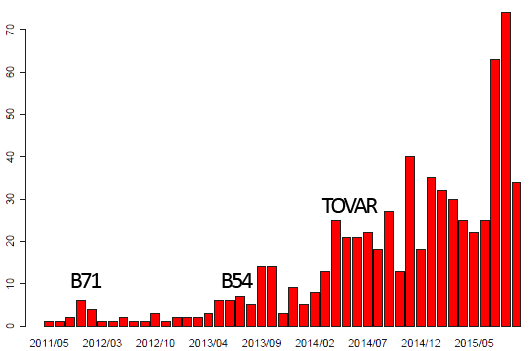
\includegraphics[height=9cm]{zeusdetection1.png}
    \caption{Detected ZeuS C\&Cs per month}
    \label{fig:detectedzeus}
\end{figure*}

\FloatBarrier
\section{Research Question}
To visualize the problem described above, it is necessary to find out the effect of botnet initiatives. Therefore, we formulate the following research question:
\begin{itemize}
\item What is the post take-down effect of botnet-initiatives on the frequency of newly set-up control and command servers?
\end{itemize}

\section{Hypotheses}
The literature review analyzed above suggests that law enforcement agencies can, in appropriate collaboration with other organizations, take down a botnet and trace back the botmaster. With the help of traceback, botmaster arrests should be made possible, causing them to leave the criminal circuit. The take-down of a certain type of botnet also shows the capabilitise of law enforcement. This should in turn startle other criminals regarding the use of certain types of malware. Therefore, we hypothesize to see a prolonged effect of botnet take-down, after a botnet initiative has taken place [H1]. We also hypothesize that collaborations with a wider variety of organizations will benefit the after-effect of botnet takedowns.

\section{Methodology}
To analyze the effect of botnet initiatives we investigate the Zeus Trojan. Zeus is the most active banking malware program to date, and thus provides us with quite some data. It is leading the market in terms of attacks as well as targeted users. In 2011 the Zeus' source code was published online, which made it possible to create new variants of the Trojan.

To analyze the long-term effect of botnet initiatives, it is necessary to obtain a set of botnet-initiatives. We will then map these events against a time-line of newly set up C\&C's, to see if a take-down event does not trigger criminals to react and neglect the initiative. For the time-line of C\&C set-ups zeustracker\footnotemark, a Zeus host tracker, will be used. The amount newly tracked C\&C's are mapped in figure \ref{fig:detectedzeus} from May 2011 to May 2015. Evidently, that means we have to establish a set of botnet initiatives against the Zeus botnet. We have defined three large botnet initiatives below and mapped them to the time-line in figure \ref{fig:detectedzeus}. The first two of these initiatives feature Microsoft working together with only a handful of financial organizations. Whether the last one, TOVAR, features collaboration with a large set of parties.

\footnotetext{found on https://zeustracker.abuse.ch/}

\subsection{B71 take-down}
In March 2012 Microsoft initiated their first attack against the Zeus botnet. The attack, named operation b71 was aimed at Zeus and its SpyEye and Ice-IX variants. Microsoft collaborated with Kyrus Tech and two financial organizations to disrupt the botnets. However, it was not until 2013 that they managed to get hold of the alleged botmaster of SpyEye.

\subsection{B54 take-down}
B54 was a botnet-initiative by Microsoft, the FBI and a few banking organizations (eight in total). The attack targeted the Citadel version of the Zeus Trojan. Microsoft had been investigating the malware for over a year until they disrupted a large part of the botnet at the start of June 2013. However, officials stated that, due to its size, they did not expect the disruption to be significant.
\begin{figure*}[]
	\centering
    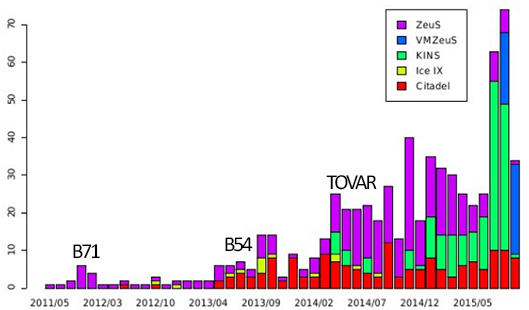
\includegraphics[height=8cm]{zeusversions1.png}
    \caption{Detected ZeuS C\&Cs per month per version}
    \label{fig:zeusversions}
\end{figure*}

\subsection{Tovar take-down}
Operation Tovar was a take-down operation conducted early in June 2014. The operation targeted the Gameover Zeus\cite{Michael2015239} botnet owned by Russian Evgeniy Bogachev. Other than regular Zeus, Game-over Zeus is a peer-to-peer botnet that has elements of the `older' Zeus Trojan. The botnet-initiative included a massive amount of 41 organisations, among which law enforcement institutions in the various countries, universities, security companies and other organizations. \FloatBarrier

By adding these three take-down events to the graph, it is possible to see how C\&C set-up before and after the initiative takes place. This makes it possible to see if the actual take-down has a significant influence on C\&C-set-up in the upcoming months. If there is a difference between the amount of parties taking part in the initiative, this will also be shown in the results.

\section{Results}
To obtain information about whether botnet take-down has effective consequences, a significant difference in C\&C set-up between the months leading up to the take-down and the months after has to be shown. Since, the data for the months around these take-downs is normally distributed we can perform a Kruskal-Wallis test. For each of the take-downs we performed a Kruskal-Wallis between the four months leading up to the take-down, and the four months following up the take-down. The results of the tests are displayed in table \ref{table:kruskal}. The test requires a significance-value of less tan 0.05 to pass. So according to Kruskal-Wallis the amount of set-up C\&C's before and after the take-down is not significant (for the chosen period of 4 months).

\begin{table}[]
\centering
\caption{Kruskal-Wallis Test for Significance}
\label{table:kruskal}
\begin{tabular}{|l|l|l|l|}
\hline
\textbf{Takedown}      & \textbf{Status} & \textbf{Mean Rank} & \textbf{Significance}  \\ \hline
\multirow{2}{*}{B71}   & Pre             & 5,75               & \multirow{2}{*}{0,122} \\ \cline{2-3}
                       & Post            & 3,25               &                        \\ \hline
\multirow{2}{*}{B54}   & Pre             & 3,40               & \multirow{2}{*}{0,243} \\ \cline{2-3}
                       & Post            & 5,50               &                        \\ \hline
\multirow{2}{*}{TOVAR} & Pre             & 4,38               & \multirow{2}{*}{0,884} \\ \cline{2-3}
                       & Post            & 4,63               &                        \\ \hline
\end{tabular}
\end{table}

Regardless of the statistical insignificance, we can see that these take-downs trigger some kind of effect. After the B54-initiative there is a sudden spike of new C\&C's for two months in a row. After doing an extra test with a two months range, rather than four, this almost resulted in a significant gain of C\&C's (significance value of 0.57). This might be a reaction from the criminal/botmaster, to get his network back online. In the case of TOVAR we see a roughly the same pattern, where there is some gain followed by a loss. The number of newly detected ZeuS C\&Cs increases again rapidly, even though the botmaster of the particular botnet was arrested. This leads us to conclude that the amount of parties has no effect either.

However, in figure \ref{fig:zeusversions} we have spit the newly detected into their particular version. Here we see something interesting. The B54-take-down was targeted at Zeus and its Ice IX variants (purple and yellow). Directly after the take-down, we see a spiky in both yellow and purple, which is in line with our previous assumption of botmaster retaliation. In the TOVAR take-down the botmaster got arrested, therefore we would expect something different. Shortly after the TOVAR take-down we see a sudden rise in KINS and later on VMZeuS. This indicates that criminals are looking for new variations of the malware, since the `old' version is apparently not feasible anymore. This leads towards the assumption that botnet initiatives with a more wide variety of organisation has a more useful effect from a technological point of view, as the botnet has almost entirely disappeared. However, the real-time effect is roughly the same, as other, possibly more advanced, types of malware come back in its place. Nontheless, these results are merely based on assumptions, and can not be proven in our current research. 

\section{Limitations}
As defined in the last section of the results, there are many factors that have not been taken into account in this paper. There is still a lot of space for future work, regarding the effects of botnet initiatives. During this project we have looked into the newly set-up C\&C's as a consequence of botnet take-down. However, it could also be interesting to look into the overall number of online C\&C's. Are the effects of botnet take-down also negligible when looking at the total number of C\&C's? Or do we actually see a downwards/upward spiral?
\footnotetext{https://www.abuse.ch/?tag=operation-b54}
\footnotetext{http://blog.fox-it.com/2012/04/12/critical-analysis-of-microsoft-operation-b71/}
Furthermore, after the B54\footnotemark and B71\footnotemark operations there was commotion about how Microsoft handles. A lot of IT companies were doing research on the Zeus botnets, when Microsoft disrupted them. Evidently, as found in our literature review, collaborative work on botnets is efficient, but it is necessary to involve the right parties. The TOVAR operation has proven this. However, it might be hard to get the right parties to work together. International cooperations might not always get along, let alone governments. Certain parties that are necessary might also lack the incentive to join in. These all limit the effect of botnet initiatives. 

Another limitation would be that information regarding the effect of botnet initiatives is scarce. In this paper we have only analyzed Zeus, but adding other malicious botnets could provide more accurate outcomes. This would provide a broader view on the issue described in this study.

Lastly, the Zeus tracker we used only acquires a subset of the real data. This gives a good insight, but the monitored size does not equal the real or estimated size of the botnets. Therefore, the amount of newly detected C\&C's is also negative skewed regarding the real value. 

\section{Conclusion}
Clearly, from the data we investigated there seems to be no significant presence between botnet set-up before and after botnet-initiatives. However, there appears to be an interesting trend among botmasters and other criminals regarding the reaction on botnet-initiatives as explain in the limitations section. Botnet-initiatives that feature a wider variety of organizations seem to have a more technologically valuable effect. As a side-effect it also evokes less of an uproar.
Essentially, wee have tried to find out whether the effect of botnet take-down has any positive real-time effects for future reference. At first glance this does not seem the case. Nontheless, we have established that the collaboration between governmental-, technical- and financial organizations has to be aligned in order to attain more positive recoil effects.\\ 


\balance
\bibliographystyle{abbrv}

\bibliography{refPaper}  

\end{document}
